\documentclass[12pt]{article}

\usepackage[margin=1in]{geometry}
\usepackage{amsmath,amsthm,amssymb}
\usepackage{mathtools}
\usepackage{mathrsfs}
\usepackage{enumitem}
\usepackage{physics}
\usepackage{tensor}

\usepackage{tikz}
\usetikzlibrary{calc,decorations.markings,patterns}

\newcommand{\magsq}[1]{\big|#1\big|^2}
\newcommand{\avg}[1]{\left<#1\right>}
\newcommand{\fullint}{\int_{-\infty}^\infty}
\newcommand{\fullintd}[1]{\fullint\dd#1\:}
\newcommand{\cint}[2]{\int_{#1}^{#2}}
\newcommand{\cintd}[3]{\cint{#1}{#2}\dd#3\:}

\begin{document}

\title{Homework 1}
\author{Sean Ericson \\ Phys 664}
\maketitle

\section*{NOTE}
In all problems the pessimistic metric (mostly minus) is used.

\section*{Problem 1 \small{(Srednicki 3.4)}}
\begin{enumerate}[label=(\alph*)]
    \item To begin, we're given
    \begin{equation} \label{1} T^{-1}(a)\phi(x)T(a) = \phi(x-a) \end{equation}
    where
    \[ T(a) = \exp(iP^\mu a_\mu) \]
    and
    \[ P^0 = H. \]
    Consider an infinitesimal $a$. Expanding the left-hand side of equation \refeq{1} (keeping terms at most linear in $a$) gives
    \begin{align*}
        T^{-1}(a)\phi(x)T(a) &= \left(\mathbb{I} - iP^\mu a_\mu\right)\phi(x)\left(\mathbb{I} + iP^\mu a_\mu\right) \\
        &= \phi(x) - iP^\mu a_\mu\phi(x) + i\phi(x)P^\mu a_\mu.
    \end{align*}
    Expanding the right-hand side, meanwhile, gives
    \[ \phi(x-a) = \phi(x) - a_\mu\partial^\mu\phi(x). \]
    Equating these expressions and canceling off the lone $\phi$ on each side yields
    \[ i\phi(x)P^\mu a_\mu - iP^\mu a_\mu\phi(x) = - a_\mu\partial^\mu\phi(x). \]
    A bit more rearrangment and canceling of the $a_\mu$ and $i$ gives us the desired result:
    \[ \boxed{\comm{\phi(x)}{P^\mu} = i\partial^\mu\phi(x)} \]

    \item Letting $\mu = 0$ in the above result gives
    \[ \comm{\phi(x)}{P^0} = i\partial^0\phi(x) \quad \implies \quad \comm{\phi(x)}{H} = i\dot{\phi}(x), \]
    which is simply the Heisenberg equation of motion for $\phi(x)$
    
    \item Consider the Heisenberg equation of motion for the time derivative of $\phi$
    \begin{equation}\label{2} \comm{\dot{\phi}(x)}{H} = i\ddot{\phi}\end{equation}
    Using the Hamiltonian for a free field
    \[ H = \frac{1}{2}\int\dd^3x \; \dot{\phi}^2(x) + \left(\nabla\phi(x)\right)^2 + m^2\phi^2(x) - 2\Omega_0, \]
    we can evaluate the left-hand side of equation \refeq{2} as follows:
    \begin{align*}
        \comm{\dot{\phi}(x)}{H} &= \frac{1}{2}\int\dd^3x' \left(\comm{\dot{\phi}(x)}{\dot{\phi}^2(x')} + \comm{\dot{\phi}(x)}{\left(\nabla\phi(x')\right)^2} + m^2\comm{\dot{\phi}(x)}{\phi^2(x')} + 2\comm{\dot{\phi}(x)}{\Omega_0} \right) \\
        &= \frac{1}{2}\int\dd^3x' \left(\comm{\dot{\phi}(x)}{\left(\nabla\phi(x')\right)^2} + m^2\comm{\dot{\phi}(x)}{\phi^2(x')}\right) \\
        &= \frac{1}{2}\int\dd^3x' \; \nabla\phi(x')\comm{\dot{\phi}(x)}{\nabla\phi(x')} + \comm{\dot{\phi}(x)}{\nabla\phi(x')}\nabla\phi(x') \\ 
        &\qquad + m^2\phi(x')\comm{\dot{\phi}(x)}{\phi(x')} + m^2\comm{\dot{\phi}(x)}{\phi(x')}\phi(x') \\  
        &= \frac{1}{2}\int\dd^3x' \; \nabla\phi(x')\nabla\comm{\dot{\phi}(x)}{\phi(x')} + \nabla\comm{\dot{\phi}(x)}{\phi(x')}\nabla\phi(x') - 2im^2\phi(x')\delta^3(x-x') \\
        &= i\int\dd^3x' \; -\nabla\phi(x')\nabla\delta^3(x-x') - m^2\phi(x')\delta^3(x-x') \\
        &= i\int\dd^3x' \; \nabla^2\phi(x')\delta^3(x-x') - m^2\phi(x')\delta^3(x-x') \\
        &= i\nabla^2\phi(x) - im^2\phi(x)
    \end{align*}
    Equating the above expression to the right-hand side of equation 2 gives
    \[ i\nabla^2\phi(x) - im^2\phi(x) = i\partial_t^2\phi(x). \]
    Some rearrangment along with combining the spatial and temporal derivatives then gives the Klein-Gordon equation:
    \[ \left(\Box + m^2\right)\phi(x) = 0 \]

    \item Define
    \[ \boldmath{P} = -\int\dd^3x\:\Pi(x)\nabla\phi(x) \]
    Then
    \begin{align*}
        \comm{\phi(x)}{\boldmath{P}} &= -\int\dd^3x'\comm{\phi(x)}{\dot{\phi}(x')\nabla\phi(x')} \\
        &= -\int\dd^3x' \; \left(\dot{\phi}(x')\comm{\phi(x)}{\nabla\phi(x')} + \comm{\phi(x)}{\dot{\phi}(x')}\nabla\phi(x') \right) \\
        &= -\int\dd^3x' \; \left(\dot{\phi}(x')\nabla\comm{\phi(x)}{\phi(x')} + \comm{\phi(x)}{\dot{\phi}(x')}\nabla\phi(x') \right) \\
        &= -i\int\dd^3x' \; \nabla\phi(x')\delta^3(x-x') \\
        &= -i\nabla\phi(x)
    \end{align*}
    which is just the spatial part of the result in part (a).

    \item By direct substitution we have that
    \begin{align*}
        P &= -\int\dd^3x\;\dot{\phi}(x)\nabla\phi(x) \\
        &= -\int\dd^3x\;\partial_t \left[\int\tilde{\dd k}\left(a(k)e^{-ikx} + a^\dag(k)e^{ikx}\right)\right]\nabla\left[\int\tilde{\dd k'}\left(a(k')e^{-ik'x} + a^\dag(k')e^{ik'x}\right)\right] \\
        &= -\int\dd^3x\; \left[\int\tilde{\dd k}(i\omega)\left(-a(k)e^{-ikx} + a^\dag(k)e^{ikx}\right)\right]\nabla\left[\int\tilde{\dd k}(i\underline{k})\left(a(k')e^{-ik'x} - a^\dag(k')e^{ik'x}\right)\right] \\
        &= -\int\dd^3x\int\tilde{\dd k}\int\tilde{\dd k'}(\omega\underline{k}') \big{(} a(k)a(k')e^{-i(k+k')x} - a(k)a^\dag(k')e^{i(k-k')x} \\ 
        &\qquad\qquad\qquad\qquad\qquad - a^\dag(k)a(k')e^{i(k-k')x} + a^\dag(k)a^\dag(k')e^{-i(k+k')x}\big{)} \\
        &= -\frac{1}{2}\int\tilde{\dd k}\int\dd k' \underline{k}'\big{(}a(k)a(k')e^{-2i\omega t}\delta^3(\underline{k}+\underline{k}') - a(k)a^\dag(k')\delta^3(\underline{k}-\underline{k}') \\
        &\qquad\qquad\qquad\qquad\qquad - a^\dag(k)a(k')\delta^3(\underline{k}-\underline{k}') + a^\dag(k)a^\dag(k')e^{2i\omega t}\delta^3(\underline{k}+\underline{k}')\big{)} \\
        &= \frac{1}{2}\int\tilde{\dd k} \; \underline{k} \left(a(k)a^\dag(k) + a^\dag(k)a(k) - a(k)a(-k)e^{-2i\omega t} - a^\dag(k)a^\dag(-k)e^{2i\omega t}\right) \\
        &= \frac{1}{2}\int\tilde{\dd k} \; \underline{k} \left(a(k)a^\dag(k) + a^\dag(k)a(k)\right) \\
        &= \frac{1}{2}\int\tilde{\dd k} \; \underline{k} \left(a(k)a^\dag(k) + a(k)a^\dag(k) - (2\pi)^32\omega\delta^3(0)\right) \\
        &= \boxed{\int\tilde{\dd k}\;\underline{k}\;a(k)a^\dag(k)}
    \end{align*}
\end{enumerate}


\section*{Problem 2 \small{(Srednicki 3.5)}}
\begin{enumerate}[label=(\alph*)]
    \item Given the Lagrangian density
    \[ \mathcal{L} = -\partial^\mu\phi^dag\partial_m\phi - m^2\phi^\dag\phi + \Omega_0 \]
    We can calculate the first variation of the action
    \[ S[\mathcal{L}] = \int\dd^4x\mathcal{L} \]
    by considering an infinitesimal variation of $\mathcal{L}$ as follows:
    \begin{align*}
        \delta S &= \int\dd^4x\left(\mathcal{L} - \delta\mathcal{L}\right) - \int\dd^4x\mathcal{L} \\
        &= \int\dd^4x \big{[} -\partial^\mu\left(\phi^\dag + \delta\phi^\dag\right)\partial_\mu(\phi + \delta\phi) - m^2\left(\phi^\dag + \delta\phi^\dag\right)\left(\phi + \delta\phi\right) + \Omega_0 \\
        &\qquad\qquad\quad - \left(-\partial^\mu\phi^dag\partial_m\phi - m^2\phi^\dag\phi + \Omega_0\right) \big{]} \\
        &= \int\dd^4x \left[-\partial^\mu\phi^\dag\partial_\mu\delta\phi - \partial^\mu\delta\phi^\dag\partial_\mu\phi - m^2\phi^\dag\delta\phi - m^2\delta\phi^\dag\phi\right] \\
        &= \int\dd^4x \left[\left(-\partial^\mu\partial_\mu\phi^\dag - m^2\phi^\dag\right)\delta\phi + \left(-\partial^\mu\partial_\mu\phi - m^2\phi\right)\delta\phi^\dag\right]
    \end{align*}
    Imposing that the variation of the action be 0 then gives
    \[ \delta S = 0 \implies -\partial^\mu\partial_\mu\phi^\dag - m^2\phi^\dag = -\partial^\mu\partial_\mu\phi - m^2\phi = 0 \]
    or
    \[ (\Box + m^2)\phi^\dag = 0 \]
    \[ (\Box + m^2)\phi = 0 \]
    Therefore, both $\phi$ and $\phi^\dag$ obey the Klein-Gordon equation.

    \item Rewriting the Lagrangian density as
    \[ \mathcal{L} = -\dot{\phi}^\dag\dot{\phi} + \nabla\phi^\dag\nabla\phi - m^2\phi^\dag\phi + \Omega_0 \]
    we can immediately read-off the conjugate momenta:
    \[ \Pi = \pdv{\mathcal{L}}{\dot{\phi}} = -\dot{\phi}^\dag \]
    \[ \Pi^\dag = \pdv{\mathcal{L}}{\dot{\phi}^\dag} = -\dot{\phi} \]
    The Hamiltonian density is then
    \begin{align*}
        \mathcal{H} &= \dot{\phi}\Pi + \dot{\phi}^\dag\Pi^\dag - \mathcal{L} \\
        &= -\Pi^\dag\Pi - \Pi\Pi^\dag + \Pi\Pi^\dag - \nabla\phi^\dag\nabla\phi + m^2\phi^\dag\phi - \Omega_0 \\
        &= \boxed{-\Pi^\dag\Pi - \nabla\phi^\dag\nabla\phi + m^2\phi^\dag\phi - \Omega_0}
    \end{align*}

    \item Given that
    \[ \phi(x) = \int\tilde{\dd k}\left(a(k)e^{-ikx} + b^\dag(k)e^{ikx}\right) \]
    we can immediately see that
    \[ \phi^\dag(x) = \int\tilde{\dd k}\left(a^\dag(k)e^{ikx} + b(k)e^{-ikx}\right) \]
    The operators $a(k)$ and $b(k)$ can then be expressed in terms of $\phi$ and $\phi^\dag$ using the result from the first problem of Homework 2:
    \begin{align*}
        a(k) &= \int\dd^3x e^{ikx}\left(i\partial_0\phi + \omega\phi\right) \\
        b(k) &= \int\dd^3x e^{ikx}\left(i\partial_0\phi^\dag + \omega\phi^\dag\right)
    \end{align*}

    \item Obviously both $a(k)$ and $b(k)$ individually follow the usually commutations relations:
    \[ \comm{a(k)}{a(k')} = \comm{a^\dag(k)}{a^\dag(k')} = 0; \qquad \comm{a(k)}{a^\dag(k)} = (2\pi)^32\omega\delta^3(\underline{k}-\underline{k}') \]
    \[ \comm{b(k)}{b(k')} = \comm{b^\dag(k)}{b^\dag(k')} = 0; \qquad \comm{b(k)}{b^\dag(k)} = (2\pi)^32\omega\delta^3(\underline{k}-\underline{k}') \]
    So we really need only consider $\comm{a}{b}$ and $\comm{a}{b^\dag}$. First consider
    \begin{align*}
        a(k)b(k') &= \int\dd^3x\int\dd^3x' \; e^{ikx}\left(i\partial_0\phi(x) + \omega\phi(x)\right)e^{ik'x'}\left(i\partial_0\phi^\dag(x') + \omega\phi^\dag(x')\right) \\
        &= \int\dd^3x\int\dd^3x' e^{i(kx + k'x')}\left(-\dot{\phi}(x)\dot{\phi}^\dag(x') + i\omega\dot{\phi}(x)\phi^\dag(x') + i\omega\phi(x)\dot{\phi}^\dag(x') + \omega^2\phi(x)\phi^\dag(x)\right)
    \end{align*}
    This implies that the commutator is given by
    \begin{align*}
        \comm{a(k)}{b(k')} &= \int\dd^3x\;\dd^3x' \; e^{i(kx + k'x')}\big{[}-\comm{\dot{\phi}(x)}{\dot{\phi}^\dag(x')} + i\omega\left(\comm{\dot{\phi}(x)}{\phi^\dag(x')} + \comm{\phi(x)}{\dot{\phi}^\dag(x')}\right) \\
        &\qquad\qquad + \omega^2\comm{\phi(x)}{\phi^\dag(x')}\big{]} \\
        &= \int\dd^3x\;\dd^3x' \; e^{i(kx+k'x')}\big{[}-\comm{\Pi^\dag(x)}{\Pi(x')} + i\omega\left(\comm{\Pi^\dag(x)}{\phi^\dag(x')} + \comm{\phi(x)}{\Pi(x')}\right) \\
        &\qquad\qquad + \omega^2\comm{\phi(x)}{\phi^\dag(x')}\big{]}
    \end{align*}
    Above, the first and last commutators are 0, while the middle two are negatives of one-another. Therefore,
    \[ \boxed{\comm{a(k)}{b(k')} = 0} \]
    Now consider
    \begin{align*}
        a(k)b^\dag(k') &= \int\dd^3x\int\dd^3x' \; e^{ikx}\left(i\partial_0\phi(x) + \omega\phi(x)\right)e^{-ik'x'}\left(-i\partial_0\phi(x') + \omega\phi(x')\right) \\
        &= \int\dd^3x\int\dd^3x' e^{i(kx - k'x')}\left(-\dot{\phi}(x)\dot{\phi}(x') + i\omega\dot{\phi}(x)\phi(x') + i\omega\phi(x)\dot{\phi}(x') + \omega^2\phi(x)\phi(x)\right)
    \end{align*}
    This implies that the commutator is given by
    \begin{align*}
        \comm{a(k)}{b^\dag(k')} &= \int\dd^3x\;\dd^3x' \; e^{i(kx - k'x')}\big{[}\comm{\dot{\phi}(x)}{\dot{\phi}(x')} + i\omega\left(\comm{\dot{\phi}(x)}{\phi(x')} + \comm{\phi(x)}{\dot{\phi}(x')}\right) \\
        &\qquad\qquad + \omega^2\comm{\phi(x)}{\phi(x')}\big{]} \\
        &= \int\dd^3x\;\dd^3x' \; e^{i(kx+k'x')}\big{[}\comm{\Pi^\dag(x)}{\Pi^\dag(x')} + i\omega\left(\comm{\Pi^\dag(x)}{\phi^(x')} + \comm{\phi(x)}{\Pi(x')}\right) \\
        &\qquad\qquad + \omega^2\comm{\phi(x)}{\phi(x')}\big{]}
    \end{align*}
    So, just as for $\comm{a(k)}{b(k')}$, we have that
    \[ \boxed{\comm{a(k)}{b^\dag(k')} = 0} \]

    \item Firstly, we have that
    \[ \phi(x) = \int\tilde{\dd k} \left(a(k)e^{-ikx} + b^\dag(k)e^{ikx}\right); \qquad \phi^\dag(x) = \int\tilde{\dd k}\left(b(k)e^{-ikx} + a^\dag(k)e^{ikx}\right) \]
    \[ \dot{\phi}(x) = i\omega\int\tilde{\dd k} \left(b^\dag(k)e^{ikx} - a(k)e^{-ikx}\right); \qquad \dot{\phi}^\dag(x) = i\omega\int\tilde{\dd k}\left(a^\dag(k)e^{ikx} - b(k)e^{-ikx}\right) \]
    \[ \nabla\phi(x) = i\int\tilde{\dd k}\; \underline{k} \left(a(k)e^{-ikx} - b^\dag(k)e^{ikx}\right); \qquad \nabla\phi^\dag(x) = i\int\tilde{\dd k} \; \underline{k} \left(b(k)e^{-ikx} - a^\dag(k)e^{ikx}\right) \]
    By direct substitution (and a bit of messy algebra which I shall not include here)
    \begin{align*}
        H &= \int\dd^3x\;\mathcal{H} \\
        &= -\Omega_0V + \int\dd^3x \; \left(-\dot{\phi}\dot{\phi}^\dag - \nabla\phi^\dag\nabla\phi + m^2\phi^\dag\phi \right) \\
        &= -\Omega_0V + \frac{1}{2\omega}\int\tilde{\dd k} \left(\omega^2 + \underline{k}^2 + m^2\right)\left(a(k)a^\dag(k) + b^\dag(k)b(k)\right) \\
        &\qquad\qquad\qquad + \frac{1}{2\omega}\int\tilde{\dd k}\left(-\omega^2 + \underline{k}^2 + m^2\right)\left(a(k)b(-k)e^{-2i\omega t} + b^\dag(k)a^\dag(-k)e^{2i\omega t}\right) \\
        &= \boxed{-\Omega_0V + \frac{\omega}{2}\int\tilde{\dd k} \left(a(k)a^\dag(k) + b^\dag(k)b(k)\right)}
    \end{align*}
    Since this is just two harmonic oscillators, $\Omega_0$ needs to be twice what it was in the text in order for the ground-state to have zero energy. I.e.
    \[ \Omega_0 = 2 \left(\frac{1}{2(2\pi)^3}\omega\int\tilde{\dd k}\right) = \boxed{\frac{1}{(2\pi)^3}\omega\int\tilde{\dd k}} \]
\end{enumerate}


\section*{Problem 3 \small{(Srednicki 7.1)}}
It is given that
\[ G(t-t') = \frac{1}{2\pi}\fullintd{E}\frac{e^{-iE(t-t')}}{-E^2 + \omega^2 - i\epsilon} \]
Firstly, to see more clearly where the poles are located, we can re-write the denominator (modulo a redfinition of $\epsilon$) as 
\[ -E^2 + \omega^2 - i\epsilon = \left((\omega - i\epsilon) - E\right)\left((\omega - i\epsilon) + E\right) \]
The poles are then located at
\[ E_+ = \omega - i\epsilon; \qquad E_- = -\omega + i\epsilon \]
By considering the cases $t<t'$ and $t>t'$ seperately, we can perform the necessary integration over $E$ as a contour integral over the complex-$E$ plane as described below:

\begin{center}
    \resizebox{250pt}{!}{
        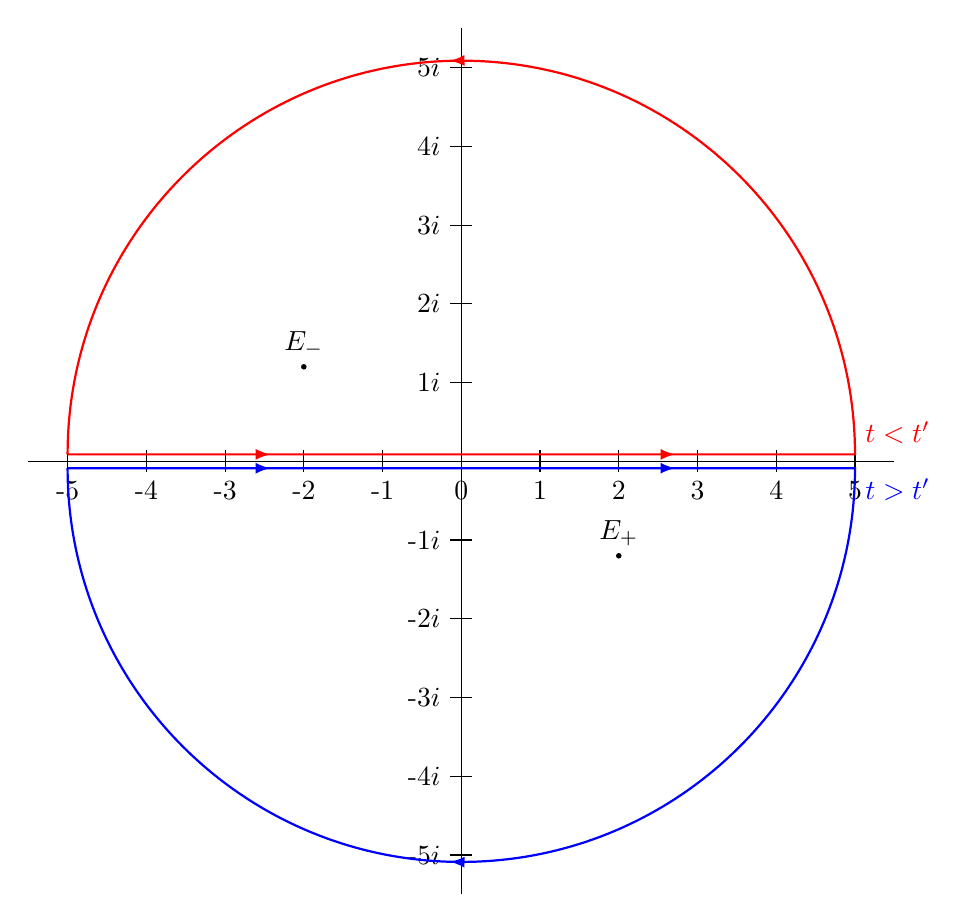
\begin{tikzpicture}
            \draw (0,-5.5) -- (0,5.5);  % Axis
            \draw (-5.5,0) -- (5.5,0);   
            \foreach \y in {-5,...,5} {
            \draw (\y,-4pt) -- (\y,4pt) node[pos=0,below] {\y};
            }
            \foreach \y in {-5,-4,-3,-2,-1,1,2,3,4,5}{
                \draw (-4pt,\y) -- (4pt,\y) node[pos=0,left] {\y $i$};
            }
            
            \node[fill,circle,inner sep=0pt, minimum width=2pt] (A) at (-2,1.2) {};
            \node[above] at (A) {$E_-$};
            \node[fill,circle,inner sep=0pt, minimum width=2pt] (A) at (2,-1.2) {};
            \node[above] at (A) {$E_+$};
            
            \draw[thick,red,yshift=2.5pt,label=test,
            decoration={ markings,  % This schema allows for fine-tuning the positions of arrows
            mark=at position 0.1 with {\arrow{latex}},
            mark=at position 0.3 with {\arrow{latex}},
            mark=at position 0.7 with {\arrow{latex}}}, 
            postaction={decorate}]
            (-5,0) -- (5,0)node[above right]{$t<t'$} arc (0:180:5);

            \draw[thick,blue,yshift=-2.5pt,label=test,
            decoration={ markings,  % This schema allows for fine-tuning the positions of arrows
            mark=at position 0.1 with {\arrow{latex}},
            mark=at position 0.3 with {\arrow{latex}},
            mark=at position 0.7 with {\arrow{latex}}}, 
            postaction={decorate}]
            (-5,0) -- (5,0)node[below right]{$t>t'$} arc (0:-180:5);
        \end{tikzpicture}
    }
\end{center}

For $t<t'$, the argument of the exponential is positive-imaginary, so we must close the contour upwards:
\[ t<t' \implies \frac{1}{2\pi}\fullintd{E}\frac{e^{-iE(t-t')}}{\left((\omega - i\epsilon) - E\right)\left((\omega - i\epsilon) + E\right)} = \frac{1}{2\pi}\fullintd{E}\frac{e^{iE(t'-t)}}{\left((\omega - i\epsilon) - E\right)\left((\omega - i\epsilon) + E\right)} \]
\[ = \frac{1}{2\pi}(-2\pi i)\frac{e^{iE_-(t'-t)}}{-2E_-} = \frac{i}{2\omega}e^{i\omega(t'-t)} \]
For $t>t'$, the argument of the exponential is negative-imaginary, so we must close the contour downwards:
\[ t>t' \implies \frac{1}{2\pi}\fullintd{E}\frac{e^{-iE(t-t')}}{\left((\omega - i\epsilon) - E\right)\left((\omega - i\epsilon) + E\right)}  \]
\[ = \frac{1}{2\pi}(2\pi i)\frac{e^{-iE_+(t-t')}}{2E_+} = \frac{i}{2\omega}e^{-i\omega(t-t')} \]
Comparing the two cases, we see that both can be expressed as
\[ \boxed{\frac{i}{2\omega}e^{-i\omega\abs{t-t'}}} \]

\section*{Problem 4 \small{(Srednicki 8.2)}}
Given that
\[ \Delta(x-x') = \frac{1}{(2\pi)^4}\int\dd^4 k \frac{e^{ik(x-x')}}{k^2 + m^2 - i\epsilon} \]
we have
\begin{align*}
    \Delta(x-x') &= \frac{1}{2\pi}\int\dd \omega \; 2\omega\int\tilde{\dd k}\frac{e^{i\omega(t-t')}e^{-i\underline{k}(\underline{x}-\underline{x}')}}{\omega^2 - \underline{k}^2 + m^2 - i\epsilon} \\
    &= \int\tilde{\dd k}e^{-i\underline{k}(\underline{x}-\underline{x}')}\frac{1}{2\pi}\int\dd \omega \frac{2\omega e^{i\omega(t-t')}}{\omega^2 - \underline{k}^2 + m^2 - i\epsilon} \\
    &= \int\tilde{\dd k}e^{-i\underline{k}(\underline{x}-\underline{x'})}\left(ie^{i\omega\abs{t-t'}}\right) \\
    &= \boxed{\int\tilde{\dd k}e^{i\omega\abs{t-t'}-i\underline{k}(\underline{x}-\underline{x'})}}
\end{align*}
where, in the second to last equality, we used the result from the previous problem (the integrals are \textit{almost} the same, with $-E^2\to\omega^2$, $\omega^2 \to m^2-\underline{k}^2$, and the factor of $2\omega$ in the numerator canceling with the one in the previous problem's denominator)

\end{document}